La figura representa un sólido del primer octante limitado por el plano vertical $y=1-x$ y la superficie $z=1-x^2$. Formule $\iiint_E f\,dV$ en los órdenes $dz\,dy\,dx$ y $dy\,dx\,dz$.

\begingroup
\shorthandoff{>}
\begin{center}
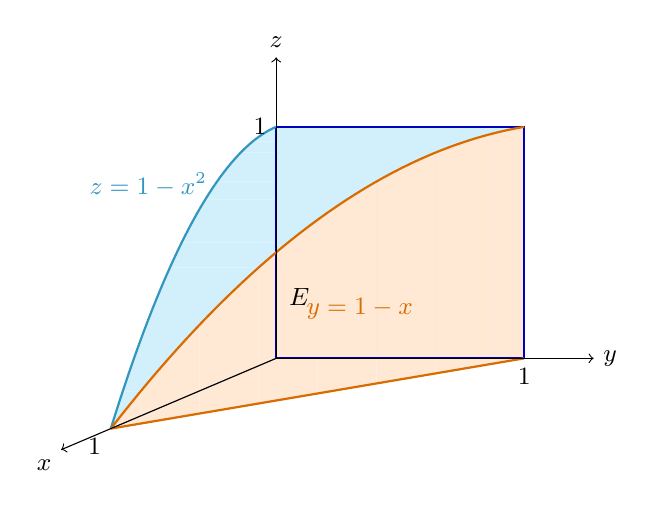
\begin{tikzpicture}[
    x={(-2cm,-.85cm)},y={(3cm,0cm)},z={(0cm,2.8cm)},
    scale=1.05,every node/.style={font=\small}]
    \fill[blue!10] (0,0,0) -- (0,1,0) -- (0,1,1) -- (0,0,1) -- cycle;
    \foreach \i in {0,...,13} {
        \pgfmathsetmacro{\xa}{\i/14}
        \pgfmathsetmacro{\xb}{(\i+1)/14}
        \fill[cyan!18]
            (\xa,0,{1-\xa*\xa}) -- (\xa,{1-\xa},{1-\xa*\xa}) --
            (\xb,{1-\xb},{1-\xb*\xb}) -- (\xb,0,{1-\xb*\xb}) -- cycle;
        \fill[orange!17]
            (\xa,{1-\xa},0) -- (\xb,{1-\xb},0) --
            (\xb,{1-\xb},{1-\xb*\xb}) --
            (\xa,{1-\xa},{1-\xa*\xa}) -- cycle;
    }
    \draw[blue!75!black,thick]
        (0,0,0) -- (0,1,0) -- (0,1,1) -- (0,0,1) -- cycle;
    \draw[cyan!75!black,thick]
        plot[domain=0:1,samples=45] (\x,0,{1-\x*\x});
    \draw[orange!85!black,thick]
        plot[domain=0:1,samples=45] (\x,{1-\x},{1-\x*\x});
    \draw[orange!85!black,thick] (0,1,0) -- (1,0,0);
    \draw[gray!65] (0,0,0) -- (1,0,0);
    \draw[->] (0,0,0) -- (1.3,0,0) node[below left] {$x$};
    \draw[->] (0,0,0) -- (0,1.28,0) node[right] {$y$};
    \draw[->] (0,0,0) -- (0,0,1.3) node[above] {$z$};
    \node[below left] at (1,0,0) {$1$};
    \node[below] at (0,1,0) {$1$};
    \node[left] at (0,0,1) {$1$};
    \node[cyan!75!black,left] at (.36,0,.86) {$z=1-x^2$};
    \node[orange!85!black,right] at (.55,.45,.38) {$y=1-x$};
    \node at (.28,.28,.35) {$E$};
\end{tikzpicture}
\end{center}
\endgroup
